% !TEX TS-program = XeLaTeX
% use the following command:
% all document files must be coded in UTF-8
\documentclass[english]{textolivre}
% build HTML with: make4ht -e build.lua -c textolivre.cfg -x -u article "fn-in,svg,pic-align"

\journalname{Texto Livre}
\thevolume{19}
%\thenumber{1} % old template
\theyear{2026}
\receiveddate{\DTMdisplaydate{2025}{9}{5}{-1}} % YYYY MM DD
\accepteddate{\DTMdisplaydate{2025}{10}{3}{-1}}
\publisheddate{\DTMdisplaydate{2026}{3}{26}{-1}}
\corrauthor{José Antonio Martínez Domingo}
\articledoi{10.1590/1983-3652.2026.61616}
%\articleid{NNNN} % if the article ID is not the last 5 numbers of its DOI, provide it using \articleid{} commmand 
% list of available sesscions in the journal: articles, dossier, reports, essays, reviews, interviews, editorial
\articlesessionname{articles}
\runningauthor{Aznar-Díaz et al.} 
%\editorname{Leonardo Araújo} % old template
\sectioneditorname{Daniervelin Pereira~\orcid{0000-0003-1861-3609}}
\layouteditorname{Saula Cecília~\orcid{0009-0006-3069-8480}}

\title{Social media as a technopedagogical tool and its effects on academic performance: a systematic review and meta-analysis}
\othertitle{Redes sociais como ferramenta tecnopedagógica e seus efeitos no desempenho acadêmico: uma revisão sistemática e meta-análise}
% if there is a third language title, add here:
%\othertitle{Artikelvorlage zur Einreichung beim Texto Livre Journal}

\author[1]{Inmaculada Aznar-Díaz~\orcid{0000-0002-0018-1150}\thanks{Email: \href{mailto:iaznar@ugr.es}{iaznar@ugr.es}}}
\author[1]{José-María Romero-Rodríguez~\orcid{0000-0002-9284-8919}\thanks{Email: \href{mailto:romejo@ugr.es}{romejo@ugr.es}}}
\author[1]{Juan-Carlos de la Cruz-Campos~\orcid{0000-0002-9263-6799}\thanks{Email: \href{mailto: juancarlosdelacruz@ugr.es}{juancarlosdelacruz@ugr.es}}}
\author[1]{José-Antonio Martínez-Domingo~\orcid{0000-0002-4976-7320}\thanks{Email: \href{mailto: josemd@ugr.es}{josemd@ugr.es}}}
\affil[1]{University of Granada, Faculty of Education Sciences, Department of Didactics and School Organization, Granada, Spain.}


\addbibresource{article.bib}
% use biber instead of bibtex
% $ biber article

% used to create dummy text for the template file
\definecolor{dark-gray}{gray}{0.35} % color used to display dummy texts
\usepackage{lipsum}
\SetLipsumParListSurrounders{\colorlet{oldcolor}{.}\color{dark-gray}}{\color{oldcolor}}

% used here only to provide the XeLaTeX and BibTeX logos
\usepackage{hologo}

% if you use multirows in a table, include the multirow package
\usepackage{multirow}

% provides sidewaysfigure environment
\usepackage{rotating}

% CUSTOM EPIGRAPH - BEGIN 
%%% https://tex.stackexchange.com/questions/193178/specific-epigraph-style
\usepackage{epigraph}
\renewcommand\textflush{flushright}
\makeatletter
\newlength\epitextskip
\pretocmd{\@epitext}{\em}{}{}
\apptocmd{\@epitext}{\em}{}{}
\patchcmd{\epigraph}{\@epitext{#1}\\}{\@epitext{#1}\\[\epitextskip]}{}{}
\makeatother
\setlength\epigraphrule{0pt}
\setlength\epitextskip{0.5ex}
\setlength\epigraphwidth{.7\textwidth}
% CUSTOM EPIGRAPH - END

% to use IPA symbols in unicode add
%\usepackage{fontspec}
%\newfontfamily\ipafont{CMU Serif}
%\newcommand{\ipa}[1]{{\ipafont #1}}
% and in the text you may use the \ipa{...} command passing the symbols in unicode

% LANGUAGE - BEGIN
% ARABIC
% for languages that use special fonts, you must provide the typeface that will be used
% \setotherlanguage{arabic}
% \newfontfamily\arabicfont[Script=Arabic]{Amiri}
% \newfontfamily\arabicfontsf[Script=Arabic]{Amiri}
% \newfontfamily\arabicfonttt[Script=Arabic]{Amiri}
%
% in the article, to add arabic text use: \textlang{arabic}{ ... }
%
% RUSSIAN
% for russian text we also need to define fonts with support for Cyrillic script
% \usepackage{fontspec}
% \setotherlanguage{russian}
% \newfontfamily\cyrillicfont{Times New Roman}
% \newfontfamily\cyrillicfontsf{Times New Roman}[Script=Cyrillic]
% \newfontfamily\cyrillicfonttt{Times New Roman}[Script=Cyrillic]
%
% in the text use \begin{russian} ... \end{russian}
% LANGUAGE - END

% EMOJIS - BEGIN
% to use emoticons in your manuscript
% https://stackoverflow.com/questions/190145/how-to-insert-emoticons-in-latex/57076064
% using font Symbola, which has full support
% the font may be downloaded at:
% https://dn-works.com/ufas/
% add to preamble:
% \newfontfamily\Symbola{Symbola}
% in the text use:
% {\Symbola }
% EMOJIS - END

% LABEL REFERENCE TO DESCRIPTIVE LIST - BEGIN
% reference itens in a descriptive list using their labels instead of numbers
% insert the code below in the preambule:
%\makeatletter
%\let\orgdescriptionlabel\descriptionlabel
%\renewcommand*{\descriptionlabel}[1]{%
%  \let\orglabel\label
%  \let\label\@gobble
%  \phantomsection
%  \edef\@currentlabel{#1\unskip}%
%  \let\label\orglabel
%  \orgdescriptionlabel{#1}%
%}
%\makeatother
%
% in your document, use as illustraded here:
%\begin{description}
%  \item[first\label{itm1}] this is only an example;
%  % ...  add more items
%\end{description}
% LABEL REFERENCE TO DESCRIPTIVE LIST - END


% add line numbers for submission
%\usepackage{lineno}
%\linenumbers


\AtBeginBibliography{
    \setlength{\itemsep}{11pt}
    \setlength{\parsep}{0pt}
}

\begin{document}
\maketitle

\begin{polyabstract}
\begin{abstract}
The use of social networks has become increasingly frequent among students, and it has been observed that these platforms can have benefits in the teaching-learning process and improve academic performance. The aim of this systematic review was to analyze whether the use of social networks in the teaching-learning process improves the academic performance of university students. The reviewed studies, conducted between 2018 and 2022, encompass various regions and are primarily quasi-experimental, with non-probabilistic sampling and a quantitative approach, utilizing questionnaires. These studies focus on the effects of social networks on performance, hypothesizing improvements. To this end, a systematic review with meta-analysis was carried out, performing the search in the Web of Science (WoS) and Scopus databases, following the Preferred Reporting Items for Systematic Reviews and Meta-Analyses (PRISMA) statement and obtaining a final sample of eight studies for the systematic review and four studies for the meta-analysis. The results show that research is controversial on the effect of social networks on academic performance, with both positive and indifferent, and even negative, results. Specifically, the meta-analysis indicates that there is no positive effect between the use of social networks and academic performance in Higher Education. In conclusion, social networks are tools that have the potential to be used in Higher Education, however, their effect on the academic performance variable is yet to be determined, although there is research that identifies promising aspects.

\keywords{Social media\sep Academic performance\sep Higher education\sep Systematic review}
\end{abstract}

\begin{portuguese}
\begin{abstract}
O uso das redes sociais tem se tornado cada vez mais frequente entre os estudantes, e tem-se observado que essas plataformas podem trazer benefícios no processo de ensino-aprendizagem e melhorar o desempenho acadêmico. O objetivo desta revisão sistemática foi analisar se o uso das redes sociais no processo de ensino-aprendizagem melhora o desempenho acadêmico de estudantes universitários. Os estudos revisados, conduzidos entre 2018 e 2022, abrangem várias regiões e são principalmente quase-experimentais, com amostragem não probabilística e abordagem quantitativa, utilizando questionários. Esses estudos focam nos efeitos das redes sociais sobre o desempenho, hipotetizando melhorias. Para isso, foi realizada uma revisão sistemática com meta-análise, executando a busca nas bases de dados Web of Science (WoS) e Scopus, seguindo a declaração Preferred Reporting Items for Systematic Reviews and Meta-Analyses (PRISMA) e obtendo uma amostra final de oito estudos para a revisão sistemática e quatro estudos para a meta-análise. Os resultados mostram que a pesquisa é controversa quanto ao efeito das redes sociais sobre o desempenho acadêmico, apresentando resultados positivos, indiferentes e até mesmo negativos. Especificamente, a meta-análise indica que não há efeito positivo entre o uso das redes sociais e o desempenho acadêmico no Ensino Superior. Em conclusão, as redes sociais são ferramentas que têm potencial para serem utilizadas no Ensino Superior; no entanto, seu efeito sobre a variável desempenho acadêmico ainda precisa ser determinado, embora existam pesquisas que identifiquem aspectos promissores.

\keywords{Redes sociais\sep Desempenho acadêmico\sep Ensino superior\sep Revisão sistemática}
\end{abstract}
\end{portuguese}
% if there is another abstract, insert it here using the same scheme
\end{polyabstract}

\section{Introduction}
The use of mobile devices and social networks among university students is increasing, facilitating ubiquitous learning and being utilized as educational tools \cite{suarezlantaron2022}. This trend has led educators to further integrate Information and Communication Technologies (ICT) in the classroom to improve students’ competencies \cite{salasrueda2019analisis}.

In the digital era, social networks like Facebook, Instagram, TikTok, and WhatsApp are transforming socialization and knowledge sharing. Social media are defined as online platforms that facilitate interaction, communication, and the exchange of knowledge. These include social networking sites (e.g., Facebook, Instagram), microblogging platforms (e.g., Twitter), and messaging applications (e.g., WhatsApp) \cite{lee2023, shafiq2023}. The impact of these platforms on education has prompted studies on their influence on academic performance \cite{alfaris2018, asiedu2017}. Academic performance is evaluated through indicators such as aptitude tests, grades, and courses passed \cite{gonzalezvalenzuela2019}.

For instance, \textcite{suarezlantaron2022} found that although WhatsApp was not designed for educational purposes, it offers educational benefits. \textcite{aiyende2021} also highlighted the positive role of social networks in academic performance and study habits. Therefore, social networks are being studied for their impact on learning and academic achievement \cite{lee2023}.

Recognizing the relevance of this topic, the objective of this study is to analyze whether the use of social networks in the teaching-learning process improves the academic performance of university students. This work is conducted as a systematic review and meta-analysis, which allows for a comprehensive synthesis of existing evidence and a rigorous evaluation of the findings reported in previous research. Furthermore, the study addresses a research gap by clarifying whether social networks truly enhance academic performance, given that prior results remain contradictory.

Thus, specific questions related to the stated objective are formulated to serve as a guide for directing the research and obtaining precise and concrete answers. The research questions posed are:

\begin{description}
    \item[RQ1:] What are the notable aspects of the studies analyzed (type of publication, temporal and geographical distribution, sample selection process, group formation, research methods, and instruments used) regarding social networks in education? 
    \item[RQ2:] What was the purpose of studies on social networks in Higher Education? 
    \item[RQ3:] What are the main characteristics of teaching through social networks in Higher Education (social networks used, duration, spaces where it occurs, intervention process, resources, techniques, and activities)?
    \item[RQ4:] What evidence exists on the effective use of social networks to improve academic performance in Higher Education?
\end{description}


\section{Method}

\subsection{Procedure}
A systematic literature review methodology was used to provide an overview of the current state of knowledge on a specific topic, following the quality criteria of the PRISMA statement \cite{page2021}. Research questions were formulated, literature was searched using a defined search equation, and quality and selection criteria were established. Additionally, a flowchart was developed to indicate the obtained and filtered results, and a meta-analysis was conducted \cite{tawfik2019}.

A search equation was created based on key terms relevant to the study topic, namely: (``Social media'' OR ``social networks'' OR ``social networking site'' OR Instagram OR Facebook OR Twitter OR WhatsApp OR YouTube OR Snapchat OR Twitch OR WeChat) AND (``higher education'' OR ``further education'' OR ``higher learning'' OR ``post-secondary education'' OR ``advanced education'' OR ``college education'' OR ``university students'') AND (``academic achievement'' OR ``learning performance'' OR ``academic performance'').

The search was restricted to the Web of Science (WoS) and Scopus databases, due to their high impact according to the Journal Citation Reports (JCR) and Scimago Journal Rank (SJR) indices and their rigorous indexing of peer-reviewed scientific articles that meet WoS and Scopus requirements. Specifically, the WoS search included the Science Citation Index Expanded (SCIE), Social Sciences Citation Index (SSCI), Arts \& Humanities Citation Index (AHCI), and the Emerging Sources Citation Index (ESCI). Additionally, a complementary search was performed in other databases to broaden the sample and reduce fugitive literature \cite{pedrazanavarro2022}. The search included ProQuest, Google Scholar, and Dialnet, but no additional results were found.

\subsection{Review process and inclusion and exclusion criteria}
The review process followed four phases: establishing the search equation, applying inclusion and exclusion criteria, analyzing titles and abstracts, and reading the full text. The inclusion and exclusion criteria are detailed in Tables \ref{tab-1} and \ref{tab-2}, and the selection process is shown in the flowchart (Figure \ref{fig-1}).

%--- codigo da tabela 1 ---%
\begin{table}[htbp]
\centering
\begin{threeparttable}
\caption{Established selection criteria.}\label{tab-1}
\begin{tabular}{p{0.47\textwidth} p{0.47\textwidth}}
\toprule
Inclusion criteria (IN) & Exclusion criteria (EX) \\
\midrule

IN1. Publications must be journal articles. &
EX1. Excludes other types of publications, such as book chapters and conference proceedings. \\

IN2. The variable measured is academic performance linked to the use of social networks. &
EX2. Academic performance is not specified as a research construct. \\

IN3. Use of social networks as a teaching-learning resource. &
EX3. Studies using resources other than social networks for the teaching-learning process. \\

IN4. The sample focuses on university students. &
EX4. The study population is non-university students. \\

IN5. Studies with an experimental or quasi-experimental design. &
EX5. Theoretical or review studies. \\
\bottomrule
\end{tabular}
\source{Own elaboration.}
\end{threeparttable}
\end{table}

%--- codigo da tabela 2 ---%
\begin{longtable}{p{0.19\textwidth} p{0.75\textwidth}}

\caption{Justification for each pair of inclusion-exclusion criteria.}\label{tab-2} \\

\toprule
Pair of criteria & Justification for implementation \\
\midrule
\endfirsthead

\endhead

IN1 – EX1 &
Peer-reviewed journal articles are prioritized, as they undergo a rigorous review process, ensuring higher quality and reliability \cite{ioannidis2022}. Sources other than journal articles, such as conference proceedings or book chapters, lack this level of review, reducing their reliability. \\

IN2 – EX2 &
Academic performance as a construct is central to the study, and only studies explicitly examining academic performance in relation to the use of social networks are considered. Excluding studies where academic performance is not a defined construct helps maintain focus on measurable outcomes directly relevant to the research objectives. \\

IN3 – EX3 &
The study focuses on evaluating the specific role of social networks in the teaching-learning process; therefore, any study using other resources (such as e-learning platforms, traditional methods, or offline resources) does not align with the research objectives. This exclusion narrows the sample to studies that solely focus on social networks as a pedagogical tool. \\

IN4 – EX4 &
University students are the population of interest due to the academic demands and social network usage patterns characteristic of this educational level. Excluding non-university populations maintains a homogeneous sample, increasing the relevance of the findings for the Higher Education context. \\

IN5 – EX5 &
Experimental and quasi-experimental designs allow for clearer causal inferences between social network use and academic performance. The exclusion of theoretical or review studies ensures that only empirical findings contribute to the meta-analysis, supporting a more data-based synthesis of results. \\

\bottomrule
\source{Own elaboration.}
\end{longtable}

%--- codigo da figura 1 ---%
\begin{figure}[h!]
\centering
\begin{minipage}{.85\textwidth}
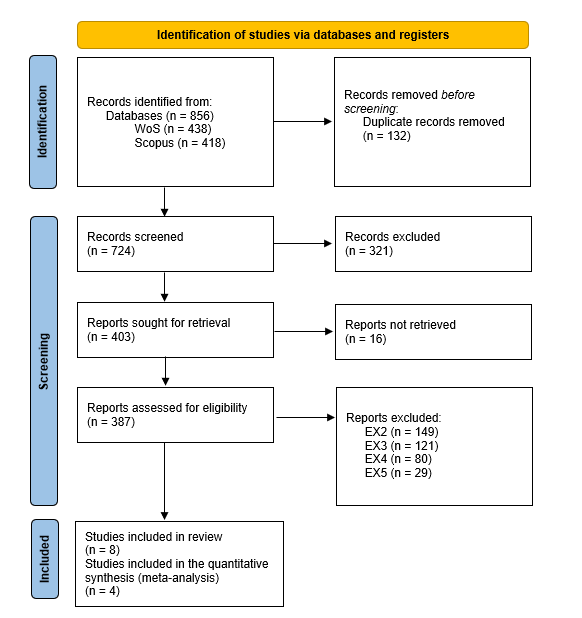
\includegraphics[width=\textwidth]{Imagens/Fig-001.png}
\caption{Flow Diagram.}
\label{fig-1}
\source{Own elaboration.}
\end{minipage}
\end{figure}

The initial results from the WoS and Scopus databases were ($n = 856$). After applying the inclusion and exclusion criteria in phases, the final sample consisted of ($n = 8$) for the systematic review and ($n = 4$) for the meta-analysis. The article search was conducted on September 15, 2023, covering documents published up to that date.


\subsection{Data analysis}
An information extraction model was used, based on substantive variables (study sample, study purposes, social networks, educational context, and activities), methodological variables (methodological design, research instruments used, and the mode of social network use), and main findings (focused on academic performance).

For the meta-analysis, articles providing information on the mean and standard deviation, derived from a comparison between a control group and an experimental group using social networks, were included. To evaluate the effectiveness of interventions using social networks, a random-effects model was selected, utilizing the Intervention Review option.

Furthermore, heterogeneity among studies was analyzed and considered high when $I^2 \geq 75\%$, medium between 50\% and 75\%, and low when $I^2 \leq 25\%$ \cite{diezbuil2023}. Through the meta-analysis, the overall effect size resulting from the different studies was obtained. Data were analyzed using the Jamovi software, version 2.3.26.

\subsection{Risk of bias assessment}
The Cochrane Collaboration’s risk of bias assessment tool was used to evaluate the risk of bias by analyzing established domains \cite{higgins2011}. Additionally, the potential for publication bias in the included studies was evaluated by inspecting the points on the funnel plot.


\section{Results}
This section delineates the principal results and salient characteristics of the studies included in the review, encompassing their research objectives, sample sizes, geographic contexts, social media platforms employed, methodological approaches, and principal outcomes pertaining to academic performance, thereby providing a rigorous and comprehensive synthesis to support comparative analysis and nuanced interpretation of the evidence (Table \ref{tab-3}).

In turn, to ensure the accuracy and transparency of the study, the analyzed studies are listed as follows:

\begin{itemize}
    \item \textcite{alexiou2020}: Being a student in the social media era: Exploring educational affordances of an ePortfolio for managing academic performance.
\item \textcite{almarzouki2022}: Social Media Usage, Working Memory, and Depression: An Experimental Investigation among University Students.
\item \textcite{demirbilek2018}: The effect of social media multitasking on classroom performance.
\item \textcite{penalba2020}: Students’ learning performance and acceptance of web 2.0 technologies based on media richness properties.
\item \textcite{perezsuasnavas2022}: Incidence of JiTTwT Methodology in the academic performance of university students.
\item \textcite{salasrueda2019}: Analysis of the use of the social network Facebook in the teaching-learning process through data science.
\item \textcite{salasrueda2018}: Use of the social network as a technological-pedagogical tool in the Higher Education teaching process.
\item \textcite{zulkifli2018}: The impact of online reciprocal peer tutoring on students’ academic performance.
\end{itemize}

%--- codigo da tabela 3 ---%
\begingroup
\scriptsize
\setlength{\tabcolsep}{3pt}

\begin{longtable}{p{0.12\textwidth} p{0.08\textwidth} p{0.13\textwidth} p{0.10\textwidth} p{0.14\textwidth} p{0.20\textwidth} p{0.12\textwidth}}

\caption{Main characteristics of analyzed studies.}\label{tab-3}

\\

\toprule
Study &
Country &
Sample Size Experimental (E) vs. Control (C) &
Research Method and Instruments &
Objective &
Teaching Characteristics &
Evidence
\\
\midrule
\endfirsthead

\textcite{alexiou2020} &
Greece &
n=123\newline
E=70; C=53 &
Quantitative\newline
Motivated Learning Strategies Questionnaire &
Identify the effect of an ePortfolio intervention using social media on self-regulated learning and academic performance &
Social Media Used: Elgg\newline
Duration: 12 weeks\newline
Spaces: ePortfolio system and a social media community\newline
Intervention Process: Three phases: forethought, performance control, and self-reflection\newline
Resources, techniques, and activities: activities using social media and ICT &
Social media use does not influence academic performance, though it improves other aspects
\\

\textcite{almarzouki2022} &
Saudi Arabia &
n=106\newline
E=54; C=52 &
Quantitative Questionnaire &
Investigate the impact of social media on working memory performance, academic performance, and negative emotional well-being (depression and anxiety) in these factors &
Social Media Used: not specified\newline
Duration: one-hour session\newline
Spaces: classroom and social media\newline
Intervention Process: procedure conducted in 5 phases\newline
Resources, techniques, and activities: tasks with social media and painting activities &
Social media use does not influence academic performance, though it increases engagement
\\

\textcite{demirbilek2018} &
Turkey &
n=122\newline
EI=41; EII=40; C=40 &
Quantitative Academic Performance Test &
Investigate whether social media sites and short messaging services, used during real-time lectures, have an effect on the academic performance of Higher Education students &
Social Media Used: Facebook\newline
Duration: 3 weeks\newline
Spaces: classroom and Facebook\newline
Intervention Process: three groups: control group (traditional), experimental group I (SMS), and experimental group II (Facebook activities)\newline
Resources, techniques, and activities: activities with Facebook (visiting profiles, accessing information and images) and discussions &
Using social media for tasks unrelated to the lesson hinders performance compared to the control group, though the experimental group improved preliminary results
\\

\textcite{penalba2020} &
Philippines &
n=100\newline
EI=34; EII=35; C=31 &
Mixed Questionnaire Interview &
Examine the influence of media richness properties on learning performance and user acceptance of web 2.0 technologies as learning tools &
Social Media Used: Facebook\newline
Duration: 8 weeks\newline
Spaces: classroom and Facebook\newline
Intervention Process: three groups: Facebook experimental group, Blogger experimental group, and control group\newline
Resources, techniques, and activities: discussion questions and activities with social media &
Social media use does not significantly influence academic performance, though it facilitates tasks
\\

\textcite{perezsuasnavas2022} &
Ecuador &
n=144\newline
E=80; C=64 &
Cross-sectional design\newline
Electronic sheet &
To determine whether student participation using Twitter during face-to-face class sessions affects the academic performance of university students &
Social Network Used: Twitter\newline
Duration: 6 weeks\newline
Spaces: the classroom and Twitter\newline
Intervention Process: the JiTTwT methodology was applied, which consists of 4 phases\newline
Resources, techniques, and activities: pre-class questions, class interaction, and Twitter engagement &
The percentage of students in the experimental group who pass the subject and improve academic performance is higher than the percentage of students in the control group
\\

\textcite{salasrueda2019} &
Mexico &
n=69\newline
E=22; CI=28; CII=19 &
Mixed Questionnaire &
Analyze Facebook use during laboratory practices and its influence on academic performance &
Social Media Used: Facebook\newline
Duration: 12 weeks\newline
Spaces: laboratory classrooms and Facebook\newline
Intervention Process: experimental group (Facebook); control groups did not use social media\newline
Resources, techniques, and activities: laboratory practices using technology and Facebook, and peer feedback &
The experimental group using Facebook achieved higher academic performance than the control group. Additionally, Facebook facilitates learning
\\

\textcite{salasrueda2018} &
Mexico &
n=69\newline
E=20; CI=29; C=20 &
Quantitative Questionnaire &
Evaluate Facebook's impact on the teaching-learning process and academic performance &
Social Media Used: Facebook\newline
Duration: 1 month\newline
Spaces: classroom and Facebook\newline
Intervention Process: experimental group used Facebook; control groups did not use social media\newline
Resources, techniques, and activities: course activities, interaction between students and teacher, sharing materials and reflections &
The experimental group using Facebook as a technopedagogical tool shows significant improvement in academic performance compared to the control group. Moreover, Facebook facilitates learning and understanding
\\

\textcite{zulkifli2018} &
Malaysia &
n=29\newline
E=29 &
Quantitative Questionnaire &
Investigate the effectiveness of online reciprocal peer tutoring on students' academic performance &
Social Media Used: Facebook\newline
Duration: 4 weeks\newline
Spaces: Facebook\newline
Intervention Process: students assigned to a single experimental group divided into 13 groups of two to three\newline
Resources, techniques, and activities: students interacted and shared information on Facebook, and participated in peer tutoring &
Facebook use in the online reciprocal peer tutoring environment significantly influenced students’ academic performance
\\

\bottomrule
\source{Own elaboration.}
\end{longtable}

\endgroup

\subsection{Substantive variables}
Regarding the study sample of the analyzed articles, sample sizes varied between 29 and 144 participants, and the studies were conducted in different countries, with no overlap in location among the investigations.

As for the purpose of the studies, all aimed to determine the effect of social networks on academic performance and learning outcomes of Higher Education students \cite{alexiou2020, almarzouki2022, demirbilek2018, penalba2020, perezsuasnavas2022, salasrueda2019, salasrueda2018, zulkifli2018}. Among these studies, three focused specifically on improving academic performance through social networks \cite{almarzouki2022, perezsuasnavas2022, salasrueda2019}.

The main social networks identified in the analyzed studies were also noted. Facebook was the most frequently used platform, serving as a technopedagogical tool \cite{demirbilek2018, penalba2020, salasrueda2019, salasrueda2018, zulkifli2018}. Other platforms included Twitter \cite{perezsuasnavas2022}, ePortfolio with social networks (Elgg) \cite{alexiou2020}, and an unspecified social network \cite{almarzouki2022}.

The studies were conducted both in the classroom and within the social network itself \cite{alexiou2020, almarzouki2022, demirbilek2018, penalba2020, perezsuasnavas2022, salasrueda2019, salasrueda2018}, except for one study where learning took place solely within the social network \cite{zulkifli2018}.

The activities and resources used in studies involving social networks focused on the experimental group, as the control group continued with traditional teaching methods without the use of social networks. The primary activities implemented were:

\begin{itemize}
    \item Microblogging tools, calendar updates, discussion spaces, management of learning identity, professional trajectory design, and performance enhancement \cite{alexiou2020}.
\item Course-related assignments \cite{almarzouki2022}.
\item Activities conducted with Facebook (visiting profiles, accessing information and images) and debates \cite{demirbilek2018}.
\item Discussion questions posted in the social network-mediated learning environment and pre- and post-tests to assess knowledge levels \cite{penalba2020}.
\item Pre-class questions, in-class interaction, and student participation on Twitter through comments and reflections on the topic covered \cite{perezsuasnavas2022}.
\item Laboratory practices using technology and Facebook as the main platform, sources and images for web design, hyperlinks, animated images, forms, and databases, as well as publishing work and comments among students \cite{salasrueda2019}.
\item Subject-specific activities, interaction between students and the instructor, and sharing of materials and reflections \cite{salasrueda2018}.
\item Students interacted and shared information on Facebook, taking on roles as tutors and tutees \cite{zulkifli2018}.
\end{itemize}

Thus, the predominant tasks across all studies included debates, answering questions, information sharing, comments, reflections, and interaction among students and with the instructor.

\subsection{Methodological variables}
The quasi-experimental methodological design was common across all studies, featuring both experimental and control groups, except for the study by \textcite{zulkifli2018}, which included only an experimental group. The sampling method was non-probabilistic, working with specific samples from university courses and degree programs.

Regarding the research method and instruments, the quantitative method predominated, utilizing questionnaires or tests \cite{alexiou2020, almarzouki2022, demirbilek2018, salasrueda2018, zulkifli2018}. Other studies employed a mixed method, using both questionnaires and interviews as research instruments \cite{penalba2020, salasrueda2019}. Additionally, a cross-sectional study was conducted using an electronic sheet based on teachers’ personal records, which included information on grades, participation, gender, enrollment, final status, among others \cite{perezsuasnavas2022}. 

The interventions using social networks varied in duration: 12 weeks \cite{alexiou2020, salasrueda2019}, 8 weeks \cite{penalba2020}, 6 weeks \cite{perezsuasnavas2022}, 4 weeks \cite{salasrueda2018, zulkifli2018}, 3 weeks \cite{demirbilek2018}, and 1 day \cite{almarzouki2022}.

With respect to the interventions carried out in the studies, these can be grouped into phase-based and non-phase-based interventions. The former were conducted as follows:

\begin{itemize}
    \item \textcite{alexiou2020}: three phases: foresight, performance control, and self-reflection.
\item \textcite{almarzouki2022}: five phases: first, the experimental group used social networks while the control group engaged in painting activities, followed by a working memory questionnaire. Then, tasks were exchanged, and the questionnaire was repeated, concluding with additional questionnaires on different variables.
\item \textcite{perezsuasnavas2022}: the JiTTwT methodology was applied, which includes four phases: 1) students answer questions before class; 2) the instructor reviews the responses and adapts the class; 3) an interactive class is conducted to clarify doubts and delve deeper into topics; 4) students reflect on what they learned and optionally participate on Twitter, without receiving rewards.
\end{itemize}
\medskip

Non-phase-based interventions were developed as follows:

\begin{itemize}
    \item \textcite{demirbilek2018}: three groups were formed: the control group, which used traditional instruction methods without technology; experimental group I, which communicated via text messages with assistants; and experimental group II, which conducted activities on Facebook during the lesson.
\item \textcite{penalba2020}: participants were assigned to three groups: a Facebook experimental group, a Blogger experimental group, and a control group, all working with the same content, while the experimental groups received identical guidance on learning technologies in social networks.
\item \textcite{salasrueda2019}: the experimental group constructed websites and used Facebook to share, debate, and reflect, while the control groups did not use social networks.
\item \textcite{salasrueda2018}: the experimental group used Facebook for course activities and reflections, while the control group did not utilize social networks.
\item \textcite{zulkifli2018}: students were randomly assigned into 13 groups of two or three people. Additionally, they completed four critical thinking tasks in the Facebook group over four weeks.
\end{itemize}


\subsection{Main findings focused on academic performance}
The analyzed studies present diverse results regarding the use of social networks and their effect on academic performance. On one hand, there are studies showing no positive influence on academic performance:

\begin{itemize}
    \item \textcite{alexiou2020}: The use of ePortfolios with social networks improved aspects of self-regulated learning but did not enhance academic performance.
\item \textcite{almarzouki2022}: The use of social networks did not improve grades, although it increased participation.
\item \textcite{penalba2020}: There were no significant differences in academic performance, although the use of Facebook facilitated work and increased perceived satisfaction.
\end{itemize}
\medskip

On the other hand, some studies identified that using social networks as a tool within the teaching-learning process improves academic performance:

\begin{itemize}
\item \textcite{perezsuasnavas2022}: The experimental group showed a greater improvement in academic performance than the control group.
\item \textcite{salasrueda2019}: The group using Facebook had a higher average in projects and better communication.
\item \textcite{salasrueda2018}: The use of Facebook resulted in higher grades and better comprehension.
\item \textcite{zulkifli2018}: Tutoring on Facebook significantly improved students’ scores.
\end{itemize}
\medskip
Additionally, there is a study in which the use of social networks has a negative influence:

\begin{itemize}
\item \textcite{demirbilek2018}: A negative impact of social network use on academic performance was identified. When students engaged in non-class-related tasks using mobile phones and social networks, their performance was adversely affected compared to traditional note-taking with pen and paper, although there was an improvement in preliminary results.
\end{itemize}

\subsection{Meta-analysis}
Although the final sample is ($n = 8$), a meta-analysis could only be conducted on four studies \cite{demirbilek2018, penalba2020, perezsuasnavas2022, salasrueda2019}. Thus, four studies ($n = 4$) that did not provide sufficient data to calculate the effect size were excluded \cite{alexiou2020, almarzouki2022, salasrueda2018, zulkifli2018}.

Regarding the analysis, the standardized mean difference was executed as the outcome indicator. A random-effects model was used for the data (Table \ref{tab-4}). The quantification of heterogeneity, represented by $tau^2$, was calculated using the restricted maximum likelihood estimator \cite{viechtbauer2005}. Along with the $tau^2$ estimate, the Q test for heterogeneity \cite{cochran1954} and the $I^2$ statistic regarding heterogeneity are presented. In situations where some degree of heterogeneity is evident (i.e., $tau^2 > 0$, independent of the results obtained from the Q test), a prediction interval for the true outcomes is reported. To assess the possibility of outlying and/or influential studies in the model, studentized residuals and Cook’s distances were employed. Studies with a studentized residual exceeding the $100 \times (1 - .05/(2 \times k))$ percentile of a standard normal distribution are considered potential outliers (using a Bonferroni correction with a two-tailed alpha = .05 for $k$ studies included in the meta-analysis). Furthermore, studies with a Cook’s distance greater than the median plus six times the interquartile range of the Cook’s distances are identified as influential. To evaluate the asymmetry of the funnel plot, two tests are used: the rank correlation and regression tests, employing the standard error of the observed results as a predictor.
\newpage

%--- codigo da tabela 4 ---%
\begin{table}[h!]
\centering
\caption{Random Effects Model ($n = 4$).}\label{tab-4}

\begin{tabular}{p{0.10\textwidth} p{0.08\textwidth} p{0.08\textwidth} p{0.08\textwidth} p{0.08\textwidth} p{0.15\textwidth} p{0.15\textwidth}}
\toprule
 & Estimate & SE & Z & $p$ & CI Lower Limit & CI Upper Limit \\
\midrule
Intercept & -.0134 & .495 & -.0270 & .978 & -.984 & .958 \\
\bottomrule
\end{tabular}
\source{Own elaboration.}
\notes{$Tau^2$ Estimator: Restricted Maximum Likelihood; SE = Standard Error.}
\end{table}

On the other hand, the standardized mean differences observed varied between -1.3693 and 1.0485, with a majority being positive (75\%). The estimated standardized mean difference, according to the random-effects model, was -.0134 with a 95\% Confidence Interval (CI): - .9844 to .9576 (Figure \ref{fig-2}). Consequently, the average result showed no significant differences from zero ($z = -.0270, p = .9784$). The $Q$ test indicates heterogeneity in the true results ($Q3) = 43.569, p < .0001, tau^2 = .9214, I^2 = 94.3671$\% (Table \ref{tab-5}). A 95\% prediction interval for the true results is provided (-2.1305 to 2.1037). Although the estimated average result is negative, some studies may have true positive results. Upon examining the studentized residuals, one study \cite{demirbilek2018} was identified with a value greater than ± 2.4977, possibly being an outlier in this model. According to the Cook’s distances, none of the studies were deemed excessively influential. Both the rank correlation and regression tests did not indicate asymmetry in the funnel plot ($p = .7500$ and $p = .6971$, respectively) (Figure \ref{fig-3}).

%--- codigo da figura 2 ---%
\begin{figure}[h!]
\centering
\begin{minipage}{.85\textwidth}

\includegraphics[width=\textwidth]{Imagens/Fig2.png}
\caption{Forest plot for the academic performance variable.}
\label{fig-2}
\source{Own elaboration.}
\end{minipage}
\end{figure}

%--- codigo da tabela 5 ---%
\begin{table}[h!]
\centering
\caption{Heterogeneity statistics.}\label{tab-5}

\begin{tabular}{p{0.05\textwidth} p{0.14\textwidth} p{0.08\textwidth} p{0.08\textwidth} p{0.03\textwidth} p{0.05\textwidth} p{0.07\textwidth} p{0.08\textwidth}}
\toprule
$Tau$ & $Tau^2$ & $I^2$ & $H^2$ & $R^2$ & $Df$ & $Q$ & $p$ \\
\midrule
.960 & .9214 \newline (SE = .8016) & 94.37\% & 17.753 & . & 3.000 & 43.257 & < .001 \\
\bottomrule
\end{tabular}
\source{Own elaboration.}
\end{table}

%--- codigo da figura 3 ---%
\begin{figure}[h!]
\centering
\begin{minipage}{.85\textwidth}
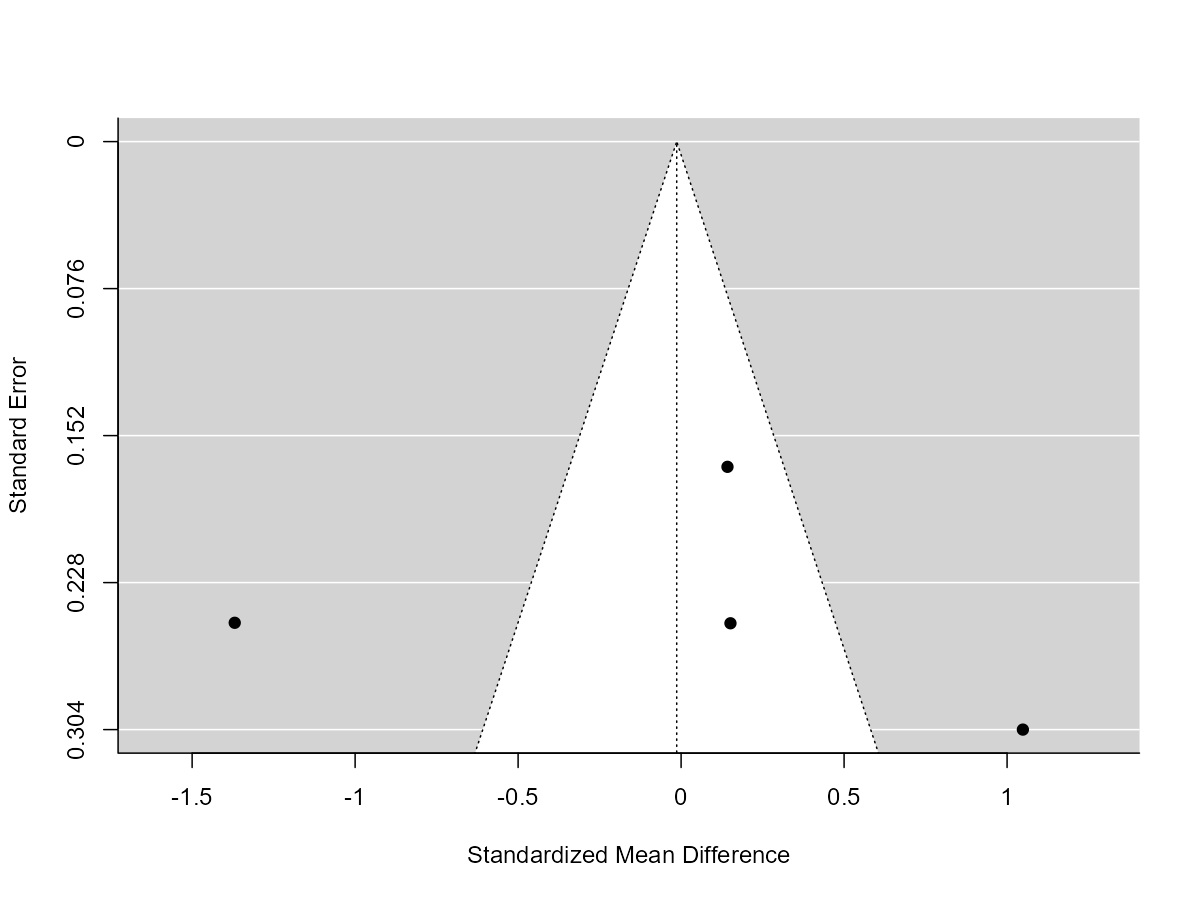
\includegraphics[width=\textwidth]{Imagens/Fig-003.png}
\caption{Funnel Plot of the Meta-Analysis on Studies of Learning Through Social Networks and Academic Performance.}
\label{fig-3}
\source{Own elaboration.}
\end{minipage}
\end{figure}

\subsection{Risk of bias in studies}
Additionally, the studies included in the meta-analysis were analyzed to assess the risk of bias (Figure \ref{fig-4} and Table \ref{tab-6}). The research conducted by \textcite{demirbilek2018} showed a high risk of bias in the domains of selection bias (allocation concealment), performance bias (blinding of participants and personnel), detection bias (blinding of outcome assessment), and attrition bias (incomplete outcome data); a low risk of bias in the domains of selection bias (random sequence generation) and reporting bias (selective reporting of results); and unclear risk in the domain of other biases (specific context of the study).

%--- codigo da figura 4 ---%
\begin{figure}[h!]
\centering
\begin{minipage}{.85\textwidth}
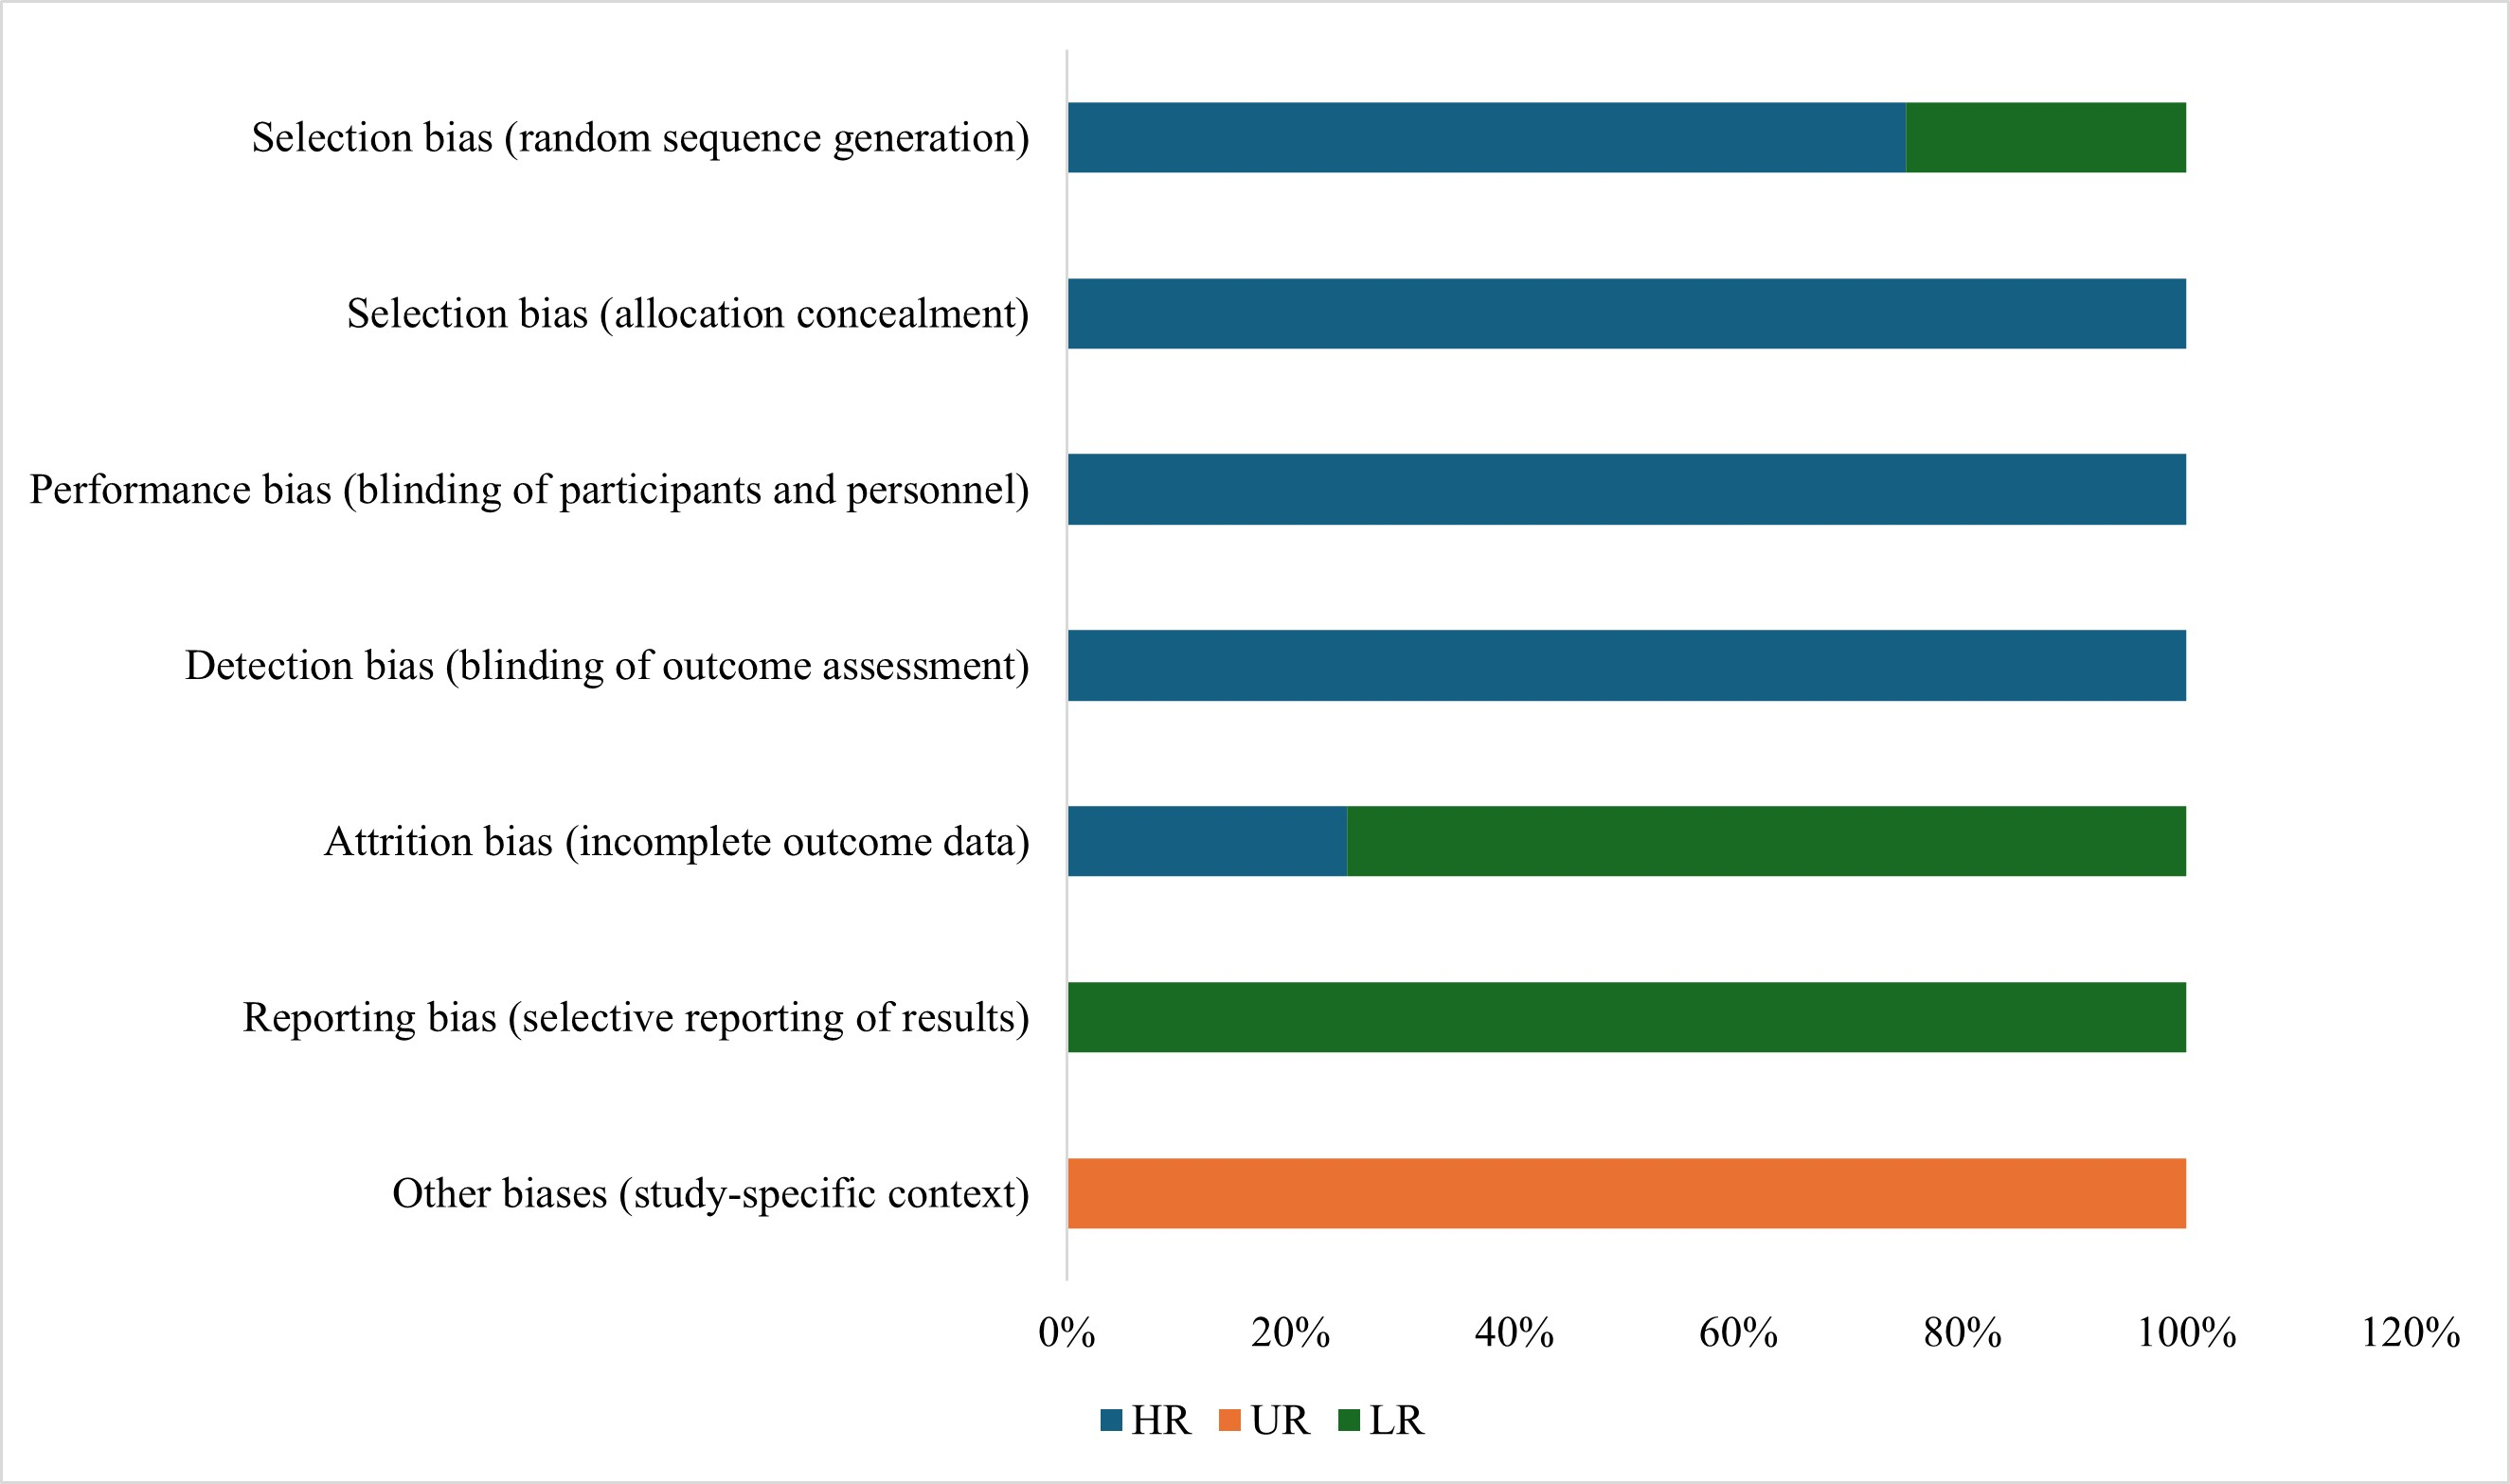
\includegraphics[width=\textwidth]{Imagens/Fig-004.jpg}
\caption{Risk of bias by domain as percentage.}
\label{fig-4}
\source{Own elaboration.}
\notes{Low Risk = LR; Unclear Risk = UR; High Risk = HR.}
\end{minipage}
\end{figure}

%--- codigo da tabela 6 ---%
\begin{table}[h!]
\centering
\small
\caption{Risk of bias by domain.}\label{tab-6}

\begin{tabular}{p{0.12\textwidth} p{0.10\textwidth} p{0.10\textwidth} p{0.10\textwidth} p{0.09\textwidth} p{0.09\textwidth} p{0.09\textwidth} p{0.08\textwidth}}
\toprule

Study &
Selection Bias (Random Sequence Generation) &
Selection Bias (Allocation Concealment) &
Performance Bias (Blinding of Participants and Personnel) &
Detection Bias (Blinding of Outcome Assessment) &
Attrition Bias (Incomplete Outcome Data) &
Reporting Bias (Selective Outcome Reporting) &
Other Biases (Study-Specific Context) \\

\midrule

\textcite{demirbilek2018} & LR & HR & HR & HR & HR & LR & UR \\

\textcite{penalba2020} & HR & HR & HR & HR & LR & LR & UR \\

\textcite{pedrazanavarro2022} & HR & HR & HR & HR & LR & LR & UR \\

\textcite{salasrueda2019} & HR & HR & HR & HR & LR & LR & UR \\

\bottomrule
\end{tabular}
\source{Own elaboration.}
\notes{Low Risk = LR; Unclear Risk = UR; High Risk = HR.}
\end{table}

The other studies conducted by \textcite{penalba2020}, \textcite{perezsuasnavas2022}, and \textcite{salasrueda2019} presented the same results, which were: high bias in the domains of selection bias (random sequence generation, allocation concealment), performance bias (blinding of participants and personnel), and detection bias (blinding of outcome assessment); low bias in the domains of attrition bias (incomplete outcome data) and reporting bias (selective reporting of results); and unclear bias in the domain of other biases (specific context of the study).


\section{Discussion}
The results of the meta-analysis indicate that the use of social networks in teaching does not significantly improve the academic performance of university students. Although some studies show improvements in learning and grades, these findings are inconclusive \cite{salasrueda2018, zulkifli2018}.

Regarding the social networks most used for learning, it is noteworthy that Facebook is prominent in quasi-experimental studies, aligning with the most researched educational applications, such as Instagram, TikTok, and WhatsApp \cite{lee2023}. Furthermore, to determine learning outcomes through social networks, grades and questionnaires were the primary assessment instruments, consistent with other quantitative studies \cite{asiedu2017, shafiq2023}.

As for the results of the studies, some report improvements in academic performance \cite{perezsuasnavas2022, salasrueda2019, salasrueda2018, zulkifli2018}, supporting the positive relationship between the use of social networks and academic performance \cite{asiedu2017, lee2023, shafiq2023}. For their part, \textcite{aiyende2021} also highlight the effective role of social networks in academic performance and study habits.

These positive indicators may encourage the use of ICT in the classroom. As \textcite{salasrueda2019} point out, teachers should integrate social networks when planning academic tasks to foster technological competencies in students.

On the other hand, other studies do not find an influence on academic performance \cite{alexiou2020, almarzouki2022, penalba2020}, consistent with research that sees no link between social networks and performance \cite{alfaris2018, suarezlantaron2022}.

Focusing on the meta-analysis, it shows that the overall effect size is not statistically significant in favor of the experimental group. Thus, current studies with experimental or quasi-experimental designs indicate that the use of social networks as technopedagogical tools does not influence academic performance. However, performance is significant for the experimental group in the study by \textcite{demirbilek2018}, while in the study by \textcite{salasrueda2019}, it is the control group that shows an improvement.

Regarding the assessment of risk of bias, the four studies reviewed present a high risk of bias, possibly due to the quasi-experimental design with nonequivalent groups, lack of allocation concealment, absence of blinding of participants, personnel, and evaluators, as well as small sample sizes in some cases, variability in the duration of interventions, and the specific context of each study, which limits generalization. These problems, common in non-randomized studies, affect the validity and reliability of the results \cite{villarrealescorcia2021}.

\section{Conclusions}
The use of social networks in education is on the rise, but its impact on academic performance in Higher Education is inconclusive. The reviewed studies, conducted between 2018 and 2022, encompass various regions and are primarily quasi-experimental, with non-probabilistic sampling and a quantitative approach, utilizing questionnaires. These studies focus on the effects of social networks on performance, hypothesizing improvements.

Regarding the main characteristics of teaching through social networks in Higher Education, it is noteworthy that Facebook is the most used network, and interventions are carried out in phases or through control and experimental groups, with a variable duration ranging from one day to 12 weeks. Activities include discussions, comments, questions, reflections, and collaboration between students and teachers.

The research presents varied results: some studies show a positive, indifferent, or even negative impact on performance, although the use of networks also facilitates access to information, communication, and collaboration in learning.

The main limitations of this study center on the limited research on the relationship between social networks and academic performance, resulting in a small sample size. Moreover, the meta-analysis only included four studies due to the lack of previous research, so the results should be interpreted with caution, and further research is recommended to establish solid conclusions.

In light of this limitation, a quasi-experimental design is proposed for future studies to examine how networks impact areas such as communication, collaboration, and performance in Higher Education.

In conclusion, social networks are tools that have the potential to be employed in Higher Education; however, their effect on academic performance is still to be determined, although there are studies that identify promising aspects.

% Adjust spacing in the bibliography section


\printbibliography\label{sec-bib}
% if the text is not in Portuguese, it might be necessary to use the code below instead to print the correct ABNT abbreviations [s.n.], [s.l.]
%\begin{portuguese}
%\printbibliography[title={Bibliography}]
%\end{portuguese}


%full list: conceptualization,datacuration,formalanalysis,funding,investigation,methodology,projadm,resources,software,supervision,validation,visualization,writing,review
\begin{contributors}[sec-contributors]
\authorcontribution{Inmaculada Aznar-Díaz}[projadm,resources,software,supervision,funding]
\authorcontribution{José-María Romero-Rodríguez}[methodology,formalanalysis,visualization,datacuration,investigation,validation]
\authorcontribution{Juan-Carlos de la Cruz-Campos}[datacuration,investigation,validation]
\authorcontribution{José-Antonio Martínez-Domingo}[conceptualization,writing,review,datacuration,investigation,validation]
\end{contributors}

\section*{Acknowledgements}
This work was funded with public funds through a competitive public contract of the Andalusian Knowledge System of the Regional Government of Andalusia (Reference: PREDOC\_01759). The study derives from the Ph.D. Thesis of Martínez-Domingo, J. A. ``Redes Sociales para la mejora del aprendizaje y la competencia digital docente en comunicación y colaboración en maestros en formación'' (University of Granada). In addition, the publication of this article was supported by the Unit of Excellence of the Melilla Campus of the University of Granada, Spain (UECUMEL; Reference: UCE-PP2024-02).

\begin{dataavailability}
\txtdataavailability{databody} % options: dataavailable, dataonly, databody, datanotav, nodata
\end{dataavailability}

\end{document}

